\documentclass[parskip=half, titlepage=firstiscover, captions=tableheading, bibliography=totoc]{scrartcl}
%optionen immer variieren tabelheading bei tabellen
%ohne parskip nur einrücken
%draft macht hüllen von bilder selbst wenn sie nicht existieren um einfach zeit bei compilieren zu sparen
%\usepackage{scrhack} % nach \documentclass
\usepackage{float}
\floatplacement{figure}{htbp}
\floatplacement{table}{htbp}
\usepackage[aux]{rerunfilecheck}
\usepackage{polyglossia}
\usepackage{biblatex}
\addbibresource{Tag3.bib}%name der bib-Datei hier einfügen !
\setmainlanguage{german}
\usepackage{longtable}
\usepackage{amsmath}
\usepackage{amssymb}
\usepackage{mathtools}
\usepackage{fontspec}
\usepackage[
math-style=ISO,
bold-style=ISO,
sans-style=italic,
nabla=upright,
partial=upright,
]{unicode-math}

\setmathfont{Latin Modern Math}
\usepackage{graphicx}
\usepackage{grffile}
\usepackage[font = scriptsize, labelfont = bf,margin={10pt,10pt}]{subcaption}
\usepackage[font = scriptsize, labelfont = bf,margin={10pt,10pt}]{caption}
%anstatt margin geht auch width = 10cm
\usepackage{mleftright}
%schöneres mit  \mleft (\mright)

\setlength{\delimitershortfall}{-1sp}
%bei vielen Klammern werden sie nun größer
\usepackage[locale=DE,separate-uncertainty=true,per-mode=symbol-or-fraction]{siunitx}
\usepackage{booktabs}
\usepackage{xfrac}
\usepackage{pdflscape}
%-> dazu wäre begin{landscape} etc nötig

%nur ein beispiel zu dieser änderung wenn man will
%gleiche sachen werden bei mathe oder text anders benutzt
%\let\vaccent=\v % alten Befehl kopieren
%\RenewDocumentCommand \v {} % Befehl überschreiben
%{
%\TextOrMath{
%\vaccent % Textmodus
%}{
%\symbf % Mathemodus
%}
%}

%\NewDocumentCommand \OverfullCenter {+m} {
%\noindent\makebox[\linewidth]{#1} }
%bei zu breiten pics zentrierte ausrichtung
%zu befehl wäre dann: \OverfullCenter{\includegraphics[width=\textwidth+15pt]{figures/
%Panorama.jpg}}

\AtBeginDocument{ % wird bei \begin{document} ausgeführt
\let\symIm=\Im % werden sonst wieder von unicode-math überschrieben
\RenewDocumentCommand \Re {}
{
\operatorname{Re}
}
\let\symIm=\Im
\RenewDocumentCommand \Im {}
{
\operatorname{Im}
}
}


\usepackage{fontspec}%nach amssymb
\usepackage[unicode]{hyperref}
\usepackage[shortcuts]{extdash} % nach hyperref, bookmark am Ende!
\usepackage{bookmark}

\begin{document}

\section{Auswertung}
\label{sec:Auswertung}


Zur Veranschaulichung des Vorgangs der Wärmevverschiebung innerhalb der,
Apparatur werden zunächst beide Temperaturverläufe aufgezeichnet und es wird durch beide jeweils ein Ausgleichspolynom dritten Grades gelegt,
\begin{equation*}
p(t) = a_3t^3 + a_2t^2 + a_1t+a_0\\
\end{equation*}
mit
\begin{equation*}
\begin{aligned}[c]
a_{3,\text{warm}} &= \SI{-3,992e-3}{\kelvin\per\second\cubed}\\
a_{2,\text{warm}} &= \SI{0,1118}{\kelvin\per\second\squared}\\
a_{1,\text{warm}} &= \SI{0,8558}{\kelvin\per\second}\\  a_{0,\text{warm}} &= \SI{293,525}{\kelvin}\\
\end{aligned}
\qquad
\begin{aligned}[c]
a_{3,\text{kalt}}&= \SI{7,393e-03}{\kelvin\per\second\cubed}\\
a_{2,\text{kalt}}&= \SI{0,1912}{\kelvin\per\second\squared}\\ 
a_{1,\text{kalt}}&= \SI{-0,1619}{\kelvin\per\second}\\
a_{0,\text{kalt}}&= \SI{293,481}{\kelvin}.\\
\end{aligned}
\end{equation*}

\begin{table}[H]
\centering
\caption{Temperatur im Verlauf der Messung}
\label{tab:Dicke}
  \begin{tabular}{c c c c}
    \toprule
    $t/ \si{\minute}$ & $T_1/\si{\kelvin}$ & $T_2/\si{\kelvin}$ & $P/\si{\watt}$\\
    \midrule 
    0   &  20,6 & 19,8 & 175,0\\
    1   &  21,6 & 19,8 & 175,0\\
    2   &  22,2 & 19,8 & 175,0\\
    3   &  23,4 & 19,0 & 177,5\\
    4   &  25,3 & 17,2 & 195,0\\
    5   &  26,7 & 15,9 & 200,0\\
    6   &  28,7 & 14,0 & 202,5\\
    7   &  30,6 & 12,1 & 205,0\\
    8   &  32,6 & 10,3 & 207,5\\
    9   &  34,5 & 8,5  & 207,5\\
    10  &  36,3 & 6,8  & 210,0\\
    11  &  38,1 & 5,1  & 210,0\\
    12  &  39,8 & 3,5  & 212,5\\
    13  &  41,6 & 2,0  & 212,5\\
    14  &  43,2 & 0,8  & 212,5\\
    15  &  44,7 & 0,1  & 210,0\\
    16  &  46,2 & -0,4 & 207,5\\
    17  &  47,5 & -0,9 & 205,0\\
    18  &  48,7 & -1,3 & 205,0\\
    19  &  49,9 & -1,8 & 205,0\\
    \bottomrule
  \end{tabular}
\end{table}

\begin{figure}[H]
  \centering
  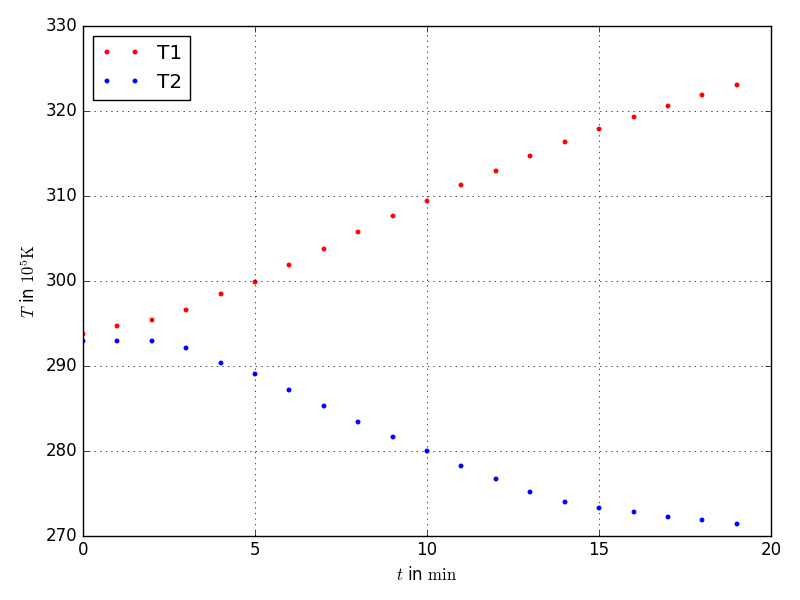
\includegraphics[width=\textwidth]{Temperatur.png}
  \caption{Temperaturverlauf der Messung kubisch interpoliert.}
  \label{fig:1}
\end{figure}

Aus den beiden Messreihen ergeben sich dann eine steigende Kurve für 
$T_1$ und eine fallende für $T_2$ und die Differentialquotienten.

Mit den Wärmekapazitäten von Wasser und der des Reservoir 1
\begin{align*}
  m_1c_W &=\SI{12600}{\joule\per\kelvin}\\
  m_kc_k &=\SI{660}{\joule\per\kelvin}\\
  \intertext{und der gemittelten Leistungsaufnahme}
  N =\SI{200,5}{Watt}
\end{align*}
kann man nun die relative Güteziffer $\nu$ berechnen

\begin{align*}
  \nu = \frac{\Delta Q_1}{N\cdot \Delta T} = \frac{m_1c_W+m_kc_k}{N}\frac{\Delta T_1}{\Delta t}.\\
\end{align*}

Für die Berechnung des Massedurchsatzes muss der an de Manometern abgelesene Zusammenhang zwischen Druck und Temperatur genutzt werden um $L$ zu bestimmen.
Die aus der linearen Ausgleichsrechnung erhaltenen Werte sind:
\begin{align*}
  &\text{Steigung } m = \num{-2520.89}
  &\text{Achsenabschnitt } b = \num{21.83}
  \intertext{und $L$ ergibt sich als}
  &L = -m\cdot R = \num{20959.86}
\end{align*}

Damit ist es nun möglich den Massendurchsatz zu berechnen:
\begin{align*}
  \frac{\Delta m}{\Delta t} &= \frac{\Delta Q_2}{L\cdot\Delta t} = \frac{m_2c_W+m_kc_k}{L}\frac{\Delta T_2}{\Delta t}\\
\end{align*}

\begin{table}[H]
\centering
\caption{Differentialquotienten in verschiedenen Punkten}
\label{tab:Dicke}
  \begin{tabular}{c c c c c}
    \toprule
    $ t/\mathrm{min}$ & $\frac{\mathrm{d}{T_1}}{\mathrm{d}{t} }/\si{\kelvin\per\second}$& $\frac{\mathrm{d}{T_1}}{\mathrm{d}{t} }/\si{\kelvin\per\second}$
    & $\nu/$ & $ \frac{\Delta m}{\Delta t}/\si{\kilogram \per\second}$ \\
    \midrule 
    4&  1,558 & -1,337 & 103.089 & 0.845 \\
    6&  1,766 &-1,658 & 116.830 & 1.049 \\
    10& 1,894 &-1,769 & 125.304 & 1.119\\
    13& 1,739 &-1,386 & 115.027 & 0.877\\
    \bottomrule
  \end{tabular}
\end{table}

Zuletzt wird aus den Werten für den Druck in den Gasleitungen noch die mechanische Kompressorleistung $N_{\text{mech}}$ berechnet.

\begin{table}
\centering
\caption{Temperatur im Verlauf der Messung}
\label{tab:Dicke}
  \begin{tabular}{c c c}
    \toprule
    $ t/\mathrm{min}$ & $p_1/\si{\pascal}$& $p_2/\si{\pascal}$\\
    \midrule 
    0   & 4.8  & 5   \\
    1   & 2.2  & 5.5 \\
    2   & 2.6  & 6.6 \\
    3   & 2.8  & 7.04\\
    4   & 3.0  & 7.6 \\
    5   & 3.1  & 8   \\
    6   & 3.2  & 8.4 \\
    7   & 3.2  & 8.75\\
    8   & 3.2  & 9.2 \\
    9   & 3.2  & 9.5 \\
    10  & 3.2  & 10.0\\
    11  & 3.2  & 10.4\\
    12  & 3.2  & 10.7\\
    13  & 3.2  & 11.1\\
    14  & 3.2  & 11.5\\
    15  & 3.2  & 11.9\\
    16  & 3.2  & 12.2\\
    17  & 3.2  & 12.5\\
    18  & 3.15 & 12.9\\
    19  & 3.15 & 13.1\\
    \bottomrule
  \end{tabular}
\end{table}






\end{document}
